\chapter{Simetrías y reglas de conservación}

\section{}

\section{}

\section{Grupo no-conmutativo: las rotaciones y el momentum angular}

Aplicar propiedades generales a problemas específicos, pero el grupo de rotaciones no es conmutativo.

Suponer un hamiltoniano $\hat{H}$ invariante ante rotaciones:

\begin{align*}
    \left[\hat{R}_{\vec{\mu}}(\alpha),\hat{H}\right]&=0\\ 
    \left[\hat{R}_{\vec{\mu}}(\alpha),\hat{U}(t)\right]&=0
\end{align*}

Tomamos una rotación de un ángulo $\alpha$ al rededor de $z$:

\begin{align*}
    \phi'(r,\theta,\phi)
        &=\hat{R}_z(\alpha)\phi(r,\theta,\phi)\\
        &=\phi(r,\theta,\phi+\alpha)
\end{align*}

Por definición de generador, el generador $\hat{L}_z$ es tal que $\hat{R}_z(\alpha)=\exp\left(-\frac{i}{\hbar}\hat{L}_z\alpha\right)$.

\subsection{Escritura vectorial}

\begin{align*}
    \hat{\vec{L}}=\hat{\vec{r}}\times\hat{\vec{p}}=
    \begin{cases}
        \hat{L}_x=\hat{y}\hat{P}_z-\hat{z}\hat{P}_y=-i\hbar(y\dd z-z\dd y)\\
        \hat{L}_y=\hat{z}\hat{P}_x-\hat{x}\hat{P}_z=-i\hbar(z\dd x-x\dd z)\\
        \hat{L}_z=\hat{x}\hat{P}_y-\hat{x}\hat{P}_y=-i\hbar(x\dd y-y\dd x)
    \end{cases}
\end{align*}

\subsection{Relaciones de conmutación}

Las relaciones de conmutación de $\hat{\vec{L}}$ están dadas por:

\begin{equation}
    \left[\hat{L}_i,\hat{L}_j\right]=i\hbar\varepsilon_{ijk}\hat{L}_k
\end{equation}

\subsection{Espacio de representaciones}

Un espacio invariante ante un grupo de transformaciones, se le llama espacio de representaciones del grupo.
Puede ser reducible si existe una suma directa de subespacios que sean invariantes ante este mismo grupo.

\subsubsection{Espacio de representaciones irreducibles de un grupo conmutativo}

\textbf{Propiedad:} Todas las representaciones irreducibles son de dimensión 1.

\subsubsection{Espacio de representaciones irreducibles de los grupos de rotación $SU(2)$ y  $SO(3)$}

Nos vamos a interesar en los generadores de rotaciones (operadores hermíticos y unitarios).

\textbf{Propiedad:}
Sean $\hat{J_x},\hat{J_y},\hat{J_z}$  operadores autoadjuntos en un espacio de Hilbert $\mathbb{H}$ que verifican el álgebra de Lie del grupo de rotaciones:

\begin{align}
    \left[J_i,J_j\right]=i\hbar\varepsilon_{ijk}\hat{J}_k
\end{align}

entonces ${\hat{\vec{J}}}^2$ conmuta con los elementos del álgebra de Lie.

\begin{align*}
    \left[{\hat{\vec{J}}}^2,\hat{J_i}\right]=0 \text{ para } i=x,y,z
\end{align*}

El espectro común de $J_z$ y $\vec{J}^2$ es de la forma:

\begin{align}
    \vec{J}^2\ket{j,m}&=\hbar^2j(j+1)\ket*{j,m}\\
    J_z\ket*{j,m}&=
\end{align}

Definimos los operadores escalón:

\begin{align*}
    J_+&=J_x+iJ_y\\
    J_-&=J_x-iJ_y
\end{align*}

Y notamos que $J_+^\dagger=J_-$

Las relaciones de conmutación:

\begin{align*}
    \left[J_+,J_-\right]&=2\hbar J_z\\
    \left[J_z,J_\pm\right]&=\pm \hbar J_{pm}\\
    \left[\vec{J}^2,J_{\pm}\right]&=0
\end{align*}

\medskip


Con $j$ fijo, los vectores $\ket*{j,m}$, con $m=-j,\cdots,j$ forman una base ortonormal $(\bra*{j,m}\ket*{j,n}=\delta_{mn})$ de un espacio vectorial $D_j$ de dimensión $j+1$ y el espacio $D_j$ es un espacio de representaciones irreducibles del grupo de rotación.

Todo espacio de representaciones del grupo de rotaciones puede descomponerse como la suma de espacios irreducibles $$H=D_{j1} \oplus D_{j2} \oplus\cdots$$ (con índices que pueden repetirse).

\bigskip

\hspace{1cm}\textbf{Nota:} Los 3 generadores $J_x,J_y,J_z$ forman una base del álgebra de Lie llamada álgebra de Lie $SO(3)$ o $SU(2)$. Los generadores $J_x,J_y,J_z$ forman otra base de la misma álgebra más interesante. A esta base se le llama descomposición de Cartan de $SU(2)$, $SO(3)$ complejificada.

Tenemos que:

\begin{align*}
    J_z\left(J_\pm \ket*{a,m}\right)
        &=\left(\left[J_z,J_\pm\right]+J_\pm J_z\right)\ket*{a,m}\\
        &=\pm \hbar J_\pm \ket*{a,m}+\hbar mJ_\pm\ket*{a,m}\\
        &=\hbar(\pm1+m)J_\pm\ket*{a,m}
\end{align*}

por otro lado,

\begin{align*}
    \vec{J}^2\left(J_\pm\ket*{a,m}\right)=J_\pm \vec{J}^2 \ket*{a,m}=\hbar^2aJ_\pm\ket*{a,m}
\end{align*}

\textbf{Nota:}

\begin{align*}
    \vec{J}^2=\frac{1}{2}\left(J_+J_-+J_-J_+\right)J_z^2
\end{align*}

Entonces notemos que:

\begin{align*}
    \hbar^2(a-m^2)
        &=\bra{a,m}\vec{J}^2-J_z^2\ket{a,m}\\
        &=-\frac{1}{2}\bra{a,m}\left(J_+J_-+J_-J_+\right)\ket{a,m}\\
        &\geq 0\\
    a&\geq m^2
\end{align*}

Existe un valor máximo de $m:m_{max}$, y por tanto un mínimo. 

Esto se traduce en:

\begin{align*}
    J_+\ket{a,m_{max}}&=0\\
    J_-\ket{a,m_{min}}&=0
\end{align*}

Por otro lado,

\begin{align*}
    \vec{J^2}
        &=J_z^2+\frac{1}{2}\left(J_+J_-+J_-J_+\right)\\
        &=J_z^2+J_+J_--\hbar J_z
\end{align*}

Aplicamos la relación a $\ket{a,m_{max}}$ y a $\ket{a,m_{min}}$:

\begin{align*}
    \vec{J}^2\ket{a,m_{max}}
        &=\hbar^2a^2\ket{a,m_{max}}\\
        &=\\
        &=\hbar^2 m_{max} (m_{max}+1)\ket{a,m_{max}}
\end{align*}

$$a^2=m_{max}(m_{max}+1)$$

de igual manera $a^2=m_{min}(m_min-1)$.

\medskip

Dado que $J_z\left(J_{\pm}\ket{a,m}\right)=\hbar(\pm1+m)(J_\pm\ket{a,m})$ podemos definir:

\begin{align}
    \ket{a,m=m\pm1}=\frac{1}{c_\pm}J_\pm\ket{a,m}
\end{align}

podemos intuir que $m_{max}=m_{min}+n$ con $n\in \mathbb{N}$ entonces:

\begin{align}
    a^2=m^2_{max}+m_{max}=m_{min}^2+m_{min}
\end{align}

De esto: $m_{min}=-\frac{n}{2}$ y por tanto $m_{max}=m_{min}+n=\frac{n}{2}=j$.

Por tanto $m=-j,-j+1,\cdots,j-1,j$ y tenemos $(2j+1)$ valores posibles.

Ahora la normalización $c_\pm$, si $\ket{j,m}$ está normalizado,

\begin{align*}
    \abs{c_{\pm}}^2\norm*{\ket{j,m+1}}^2
        &=\bra{j,m}J_-J_+\ket{j,m}\\
        &=\hbar^2 \left(j(j+1)-m(m+1)\right)
\end{align*}

de igual manera para $c_-$.

Por tanto, cada espacio $D_j$ es de dimensión $(2j+1)$ y los operadores $J_\pm$, $J_z$ actúan dentro de $D_j$ al igual que $J_x,J_y,J_z$ que se obtienen por medio de combinaciones lineales. 

$D_j$ es invariante ante rotaciones: es un espacio de representación del grupo de rotación.

Cada $D_j$ no puede descomponerse en la suma de 2 espacios. 

\hfill$\qed$

\subsection{En resumen: Representaciones irreducibles de los grupos de rotación $SO(3)$ y $SU(2)$}

Recordemos que:

\begin{align*}
    \vec{J}^2\ket{j,m}=\hbar^2j(j+1)\ket{j,m}\\
    J_z\ket{j,m}=\hbar m\ket{j,m}
\end{align*}

Vamos a tomar ahora al estado $\ket{j,m}$ y lo vamos a rotar por $2\pi$ al rededor de $z$.

\begin{align*}
    R_z(2\pi)
        &=\pm\ket{j,m}
\end{align*}

$+$ si $m$ es entero, y $-$ si $m$ es medio entero.

Entonces:

Si $D_j$ es una representación de $SO(3)$, entonces $R(2\pi)=\mathbb{I}$ $\Rightarrow j$ (y por tanto $m$ también) debe ser un entero.

$$
\rightarrow l=j=0,1,2,\cdots
$$

así, el espacio de representaciones irreducibles de $SO(3)$ son los espacios $D_l$ caracterizados por el entero $l$. Notemos que $D_l$ es de dimensión impar $(2l+1)$.

Si $D_j$ es una representación de $SU(2)$ (rotación de espín $1/2$) $\Rightarrow R(4\pi)=\mathbb{I}$, entonces los valores de $j$ permitidos son:

$$
j=0,1/2,1,\cdots
$$

Los espacios de representación irreducibles de $SU(2)$ son los espacios $D_j$ caracterizados por el entero o medio entero $j$.

\textbf{Nota:}
\begin{itemize}
    \item Del hecho que $\left[\vec{J}^2,\vec{J}\right]=0\Rightarrow\left[J^2,R\right]=0$ para cualquier operador de rotación.
    $$
    R_\mu (\theta)=\exp()
    $$
    Decimos que $\vec{J}^2$ es un operador de Casimir del grupo de rotación.
    Uno de los espacios de representación irreducibles $D_j$ es el espacio propio de $\vec{J}^2$ caracterizado por el autovalor $\hbar^2 $

    \item Los vectores $\ket{j,m}$ forman una base de $D_j$. Estos vectores son autovectores de $J_z$ y la dirección de esta base depende de la elección del eje $z$
\end{itemize}

\textbf{Ejemplos}

\begin{enumerate}
    \item Para describir el espín $1/2$, el espacio $\mathbb{H}_{espin}=\mathbb{C}^2$ de dimensión 2 y los operadores $S_x,S_y,S_z$ y se identifican con el espacio $D_{1/2}$ para $j=1/2$.
    \item El espacio $\mathbb{R}^3$ es un espacio de representaciones irreducible de $SO(3)$. $\mathbb{R}^3$ se identifica al espacio $D_{l=1}$ con base $\ket{l=1,m=-1,0,+1}$ que identificamos con $\ket{x},\ket{y},\ket{z}$ de la siguiente manera:
    \begin{enumerate}
        \item vamos a escribir
    \end{enumerate}
\end{enumerate}


\subsubsection{Aplicación: espectro de un rotor rígido:}

Tomar el ejemplo de una molécula diatómica $(HCl,NaCl,H_2,O_2,\cdots)$, vamos a ignorar la vibración de la molécula y la traslación $\Rightarrow$ solo consideramos rotaciones en ella misma:

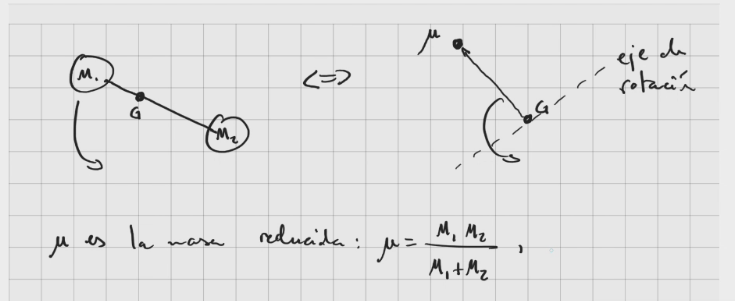
\includegraphics[width=0.4\textwidth]{Graficas/G1-Aug2.png}

\textbf{El espacio de Hilbert de los estados cuánticos:}

Movimiento reducido a una esfera $S^2$

$$
\mathbb{H}=L^2(S^2)
$$

los vectores son funciones de onda $\Psi(\theta,\phi)$ en un punto $(\theta,\phi)$ sobre la esfera.
La esfera es el espacio de configuraciones del sistema.

Denotamos por $\ket{\theta,\phi}$ al estado de la posición (delta de Dirac en el punto).

$$
\psi(\theta,\phi)=\bra{\theta,\phi}\ket{\psi}
$$

y la resolución de la identidad:

Donde $\dd\Omega$ es el ángulo sólido de la esfera.

\textbf{Operador Hamiltoniano:}

En el caso clásico:

\begin{align*}
    H=\frac{1}{2}\mu v^2=\frac{1}{2} \mu r_o^2\omega^2=\frac{L^2}{2I}
\end{align*}

con $I$ el momento de inercia $I=\mu r_o^2$ y $L$ el momentum angular.

Cuantizamos 
$$
\hat{H}=\frac{\hat{I}^2}{2I}
$$

con $\vec{L}^2=L_x^2+L_y^2+L_z^2$

\textbf{Espectro de $\hat{H}$}

Teorema: En el espacio de hilbert $\mathbb{H}=L^2(S^2)$, cada espacio de representaciones irreducibles $D_l$, $l=0,1,2,\cdots$ aparece solo una vez:

\begin{align*}
    \mathbb{H}=L^2(s^2)=\bigoplus_{l=0}^\infty D_l
\end{align*}


\subsection{Importancia de las representaciones irreducibles:}

\subsubsection{Propiedades fundamentales: el lema de Schur y el teorema de Wigner}

El lema de Schur tiene varias formulaciones, pero la más útil en mecánica cuántica es la siguiente:

\textbf{Lema de Schur:} Sea $\hat{A}:\mathbb{H}\rightarrow\mathbb{H}$ un operador que actúa sobre el espacio de Hilbert $\mathbb{H}$. Vamos a suponer que este es la suma directa de espacios irreducibles de un grupo $G$, que pos simplicidad diremos que son $2$.

\begin{equation*}
    \mathbb{H}=D_j\oplus D_k\tag{1}
\end{equation*}

y estas representaciones no son equivalentes:
$$
D_j\neq D_k
$$
Bien $j\neq k$ y además para todo $\hat{G}\in G$
$$
\left[A,G\right]=0
$$
$g$ es un grupo de simetrías de $\hat{A}$. Entonces $\hat{A}$ se escribe respecto a la descomposición $(1)$ como:

$$
\hat{A}=\begin{pmatrix}
    a_j\mathbb{I} & 0\\
    0 & a_k\mathbb{I}
\end{pmatrix}
$$

(el resultado es generalizable a la suma de más representaciones irreducibles)

\textbf{Prueba:} Para esto necesitaremos 2 lemas intermedios:

\textbf{Lema de Schur A:} Si $\hat{A}:D_j\rightarrow D_k$ es un operador lineal entre 2 espacios de representaciones irreducibles de $G$ y $\left[A,G\right]=0$ $\forall \hat{G}\in G$ entonces $A=0$ o bien $A$ es un isomorfismo $\Rightarrow D_j\approxeq D_k,j=k$

Nota: 
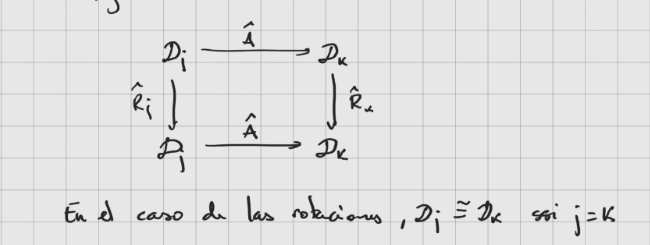
\includegraphics[width=0.4\textwidth]{Graficas/G2-Aug2.png}

\textbf{Prueba:} El Kernel de $A$, $\ker A\subset D_j$ es invariante por $G$. En efecto, si $\psi\in\ker A$, i.e. $A\psi=0$ entonces sean $\psi '=G\psi$ entonces:

\begin{align*}
    A\psi ' =AG\psi=GA\psi=0\Rightarrow\psi ' \in\ker A
\end{align*}

Ahora bien, $D_j$ es irreducible $\Rightarrow \ker A=\{0\}\Rightarrow A$ es inyectiva o $A=0$.

Por otro lado, $Im(A)\subset D_k$ es invariante por $G$. En efecto, si $\psi \in Im(A)$, $\psi=A\phi\Rightarrow\psi'\in Im(A)$ Como $D_k$ es irreducible, $Im(A)=0$ o $Im(A)=D_k$ (es sobreyectiva).

Por tanto, $A=0$ o $A$ es isomorfismo.

\textbf{Lema de Schur B:}

Si $A:D_j\rightarrow D_k$ es un operador lineal en un espacio de representaciones irreducibles de $G$ y $\left[A,G\right]=0 \forall \hat{G}\in G$ entonces $A=a\mathbb{I}$ con $a\in \mathbb{C}$

\textbf{Prueba:}
Los espacios propios de $A$ denotados $\mathbb{H}_a\subset D_j$ son invariantes por la acción de $G$. Pero $D_j$ es irreducible. Entonces solo hay uno.

El resto de la prueba se basa en escribir al operador $A$ como una matriz de $2\times 2$ utilizando proyecciones, donde los elementos de matriz $A_{ab}$ están dados por $P_a A p_b$. Y por tanto:

\begin{align*}
    \begin{pmatrix}
        a_j \mathbb{I} & 0\\
        0 & a_k \mathbb{I}
    \end{pmatrix}
\end{align*}


\textbf{Teorema de Wigner}
Si el hamiltoniano $\hat{H}$ tiene un espectro discreto y admite una simetría por un grupo de invarianza G discreto o continuo, i.e.$$\left[H,G\right]=0\forall G\in G$$

entonces genéricamente (el resultado de toda perturbación respecto a esta simetría es estable), los espacios propios de $H$ son representaciones irreducibles de $G$.

En particular, si el grupo $G$ es conmutativo, sus representaciones irreducibles son de dimensión $1$ y esperaríaos que no haya degeneración en el espectro, i.e. todos los niveles son distintos (momentum de espectro continuo),
Si el grupo es no conmutativo, entonces admite representaciones irreducibles de dimensión $d\geq 1$ y esperamos degeneraciones en el espectro de multiplicidad $d$. (i.e. distintos estados con misma energía).

\textbf{Nota:}
Esta propiedad resulta muy útil en física molecular: conociendo las representaciones irreducibles de distintos grupos (hay al menos 230 grupos finitos del espacio catalogados y observados en la naturaleza) y observando el espectro de una molécula, deducimos el grupo de invarianza y así podemos deducir la forma de la molécula (geométrica).

Espectro $\Rightarrow $ grupo de simetría $\Rightarrow$ forma de la molécula.

\textbf{Ejemplo: El espectro del átomo de hidrógeno}

\textit{Repaso:}

\begin{align*}
    \hat{H}=\frac{\hat{\vec{p}}^2}{2m}-\frac{e^2}{4\pi\epsilon_o}\frac{1}{r} 
\end{align*}

por el momento no tomamos en cuenta el espín. $\hat{H}$ es invariante ante rotaciones: $\left[\hat{H},\hat{T}\right]=0$. El espectro es tal que:

\begin{align*}
    \hat{H}\ket{\psi_{n,l,m}}=E_n\ket{\psi_{n,l,m}}   
\end{align*}


los autovectores son el producto de una función radial y de armónicos esféricos:

\begin{align*}
    \bra{x}\ket{\psi_{n,l,m}}=R_{n,l}(r)Y_{l,m}(\theta,\psi)
\end{align*}

Con $E_n=$

Cada uno de los niveles de energía constituye entonces un espacio propio 

\begin{align*}
    H_n=\bigoplus_{l=0}^{n-1}D_l
\end{align*}

Este espacio es de dimensión $n^2$

$$
\left(\sum_{l=0}^{n-1}(2l+1)=n^2\right)
$$

\textbf{Simetría adicional de Pauli, y degeneración a $l$:}

Esto pareciera contradecir el teorema de Wigner

De hecho no lo contradice, ya que el potencial tiene una forma muy particular, está en términos de $1/r$ y esto hace que haya una simetría más (descubierta por Pauli en $1925$), cuyo generador es:

\begin{align*}
    \hat{\vec{A}}=\frac{1}{2m}\left(\vec{p}\times\vec{L}-\vec{L}\times\vec{p}\right)-mK\frac{\vec{x}}{\abs{x}}
\end{align*}

con $K=\frac{e^2}{4\pi\epsilon}$ y $\vec{A}$ se conoce como el vector de Runge Lenz.

Es posible verificar que:

\begin{align*}
    \left[A,H\right]=0
\end{align*}

El grupo de simetrías es ahora $SO(4)$ de dimensión $6$ y cada espacio propio $H$ es irreducible para esta simetría.

Podemos romper esta simetría: correcciones relativistas. (rompen la simetría de $A$ pero no la invarianza rotacional)

\bigskip

\textbf{Átomo con varios electrones}

El espectro de átomos con un solo electrón ($z=2\leftarrow He^+$, $z=3\leftarrow Li^{2+}$) es lo mismo que $H$ pero sustituyendo la carga del núcleopor $Z_e$.

Ahora, si tenemos varios electrones, la situación es mucho más complicada: NO EXISTE SOLUCIÓN EXACTA. Pero se utilizan métodos de aproximación (método variacional).

Otro método: \textit{mean field theory} (método del campo medio). Considera que cada electrón es independiente pero está sometido a un potencial $V(r)$ promedio, resultado de todas las cargas: el núcleo $Z_e$ y los demás electrones.

Este potencial tiene simetría esférica, usualmente difiere de $1/r$. Esta diferencia rompe la simetría de Pauli. $\Rightarrow$ Se quita la degeneración de los estados con $l$ distinto.

\bigskip

\textbf{Efecto de un campo magnético externo:}
Tenemos un campo magnético externo $\vec{B}$: rompe la simetría esférica: le da prioridad a una dirección particular $\hat{B}$.

$\Rightarrow $ la degeneración de $m$ ya no va.

$\Rightarrow$ espectro no degenerado: efecto Zeeman.

Si el campo está en la dirección de $z$, hay una simetría de rotación en $z$.

Sin embargo, este subgrupo de simetrías forma un grupo conmutativo $\Rightarrow$ rompe la degeneración.

\bigskip

\textbf{Estructura fina e hiperfina del átomo de hidrógeno:}

El átomo de Bohr es una excelente aproximación, pero hay pequeñas correcciones por hacer.

Estos se detectaron gracias a la espectroscopía: se miden los niveles de energía con mucha precisión.

Estas correctiones se obtienen por métodos perturbativos y son mucho más pequeñas que $\varepsilon=13.6eV$.

\textit{Estructura fina:}
\begin{itemize}
    \item agregar una corrección relativista (viene de la ecuación de Dirac):
    $$
    \hat{H}_1'=-\frac{p^4}{8m^3c^2}+\frac{\pi\hbar^2}{2(mc)^2}\left(\frac{e^2}{4\pi\epsilon_o}\right)\delta(\vec{x})
    $$
    \item agregar la interacción del espín con la órbita:
    $$
    \hat{H}_2'=\frac{1}{2(mc)^2}\frac{1}{r}\dv*{v}{r}\vec{L}\cdot\vec{S}
    $$
\end{itemize}

Notemos que estas correcciones no rompen la simetría de rotación. 

$\hat{H}_2'$ enlaza a la posición con el espín. $\Rightarrow$ sólo el momentum angular total se conserva: $\vec{J}=\vec{L}+\vec{S}$.

Los resultados obtenidos dependen de $n,j$ y $l$ que corresponden a autovalores de $\vec{L}^2,\vec{J}^2$ que conmutan entre ellos y con $\hat{H}$.

\textit{Estructura hiperfina:}

Viene de enlazar los momentos magnéticos del protón y el electrón.



\section{Composición de momentum angulares}

\subsection{Partícula compuesta por dos partículas de espín $1/2$}

Por ejemplo, el núcleo del deuterio: protón y neutrón.
Un pión $\pi$ formado por $2$ quarks $\bar{\nu},\nu$ 
Un átomo de hidrógeno: protón $+$ electrón.

El espacio total de espín es:

\begin{align*}
    \mathbb{H}_{tot}=\mathbb{D}_{1/2}\otimes \mathbb{D}_{1/2}
\end{align*}

Con $\mathbb{D}_{1/2}:=\mathbb{H}_{spin}:=\mathbb{C}^2$. la bae del espacio es $\ket{+_z},\ket{-_z}$

En el espacio $\mathbb{H}_{tot }$ denotamos $\ket{++}=\ket{+_z}_1\otimes\ket{+_z}_2$.

Una base con las combinaciones de los elementos de las bases de cada partícula.

Si el sistema está aislado de su entorno (no interactúa con la órbita) $\Rightarrow$ es invariante ante rotaciones. El generador es el momentum angular total:

\begin{align*}
    \hat{\vec{S}}=\hat{\vec{S}}_1+\hat{\vec{S}}_2
\end{align*}


Y aquí, el hamiltoniano conmuta con $\hat{\vec{S}}$.

\begin{align*}
    \left[H,\vec{S}\right]=0
\end{align*}

Por ejemplo:

\begin{align*}
    \hat{H}=K\vec{S}_1\cdot \vec{S}_2
\end{align*}

De esta invarianza deducimos:

\begin{align*}
    \left[H,\vec{S}^2\right]&=0\\
    \left[H,S_z\right]&=0\\
    \left[\vec{S}^2,S_z\right]&=0\\
\end{align*}

Todos estos operadores tienen autovectores en común:

\begin{align*}
    \ket{J,M}
\end{align*}

Son tales que:

\begin{align*}
    \hat{S}_z\ket{J,M}&=M\hbar\ket{J,M}\\
    \hat{\vec{S}}^2\ket{J,M}&=\hbar^2 J\left(J+1\right)\ket{J,M}\\
\end{align*}

Objetivo: expresar la base $\ket{J,M}$ en función de $\ket{\pm,\pm}$.

\textbf{Propiedad:} Esta es la descomposición del espacio $\mathbb{H}_{tot}$ en vectores $\ket{J,M}$ ortonormales.

\begin{itemize}
    \item \textbf{Singlete}
    $$\ket{J=0,M=0}=\frac{1}{\sqrt{2}}\left(\ket{+-}-\ket{-+}\right)$$
    \item \textbf{Triplete}
    \begin{align*}
        \ket{J=1,M=1}&=\ket{++}\\
        \ket{J=1,M=0}&=\frac{1}{\sqrt{2}}\left(\ket{+-}+\ket{-+}\right)\\
        \ket{J=1,M=-1}&=\ket{--}\\
    \end{align*}
\end{itemize}

Con esto, el espacio $\mathbb{H}_{tot}$ se descompone en la suma de 2 representaciones irreducibles del grupo de rotaciones:

$$\mathbb{D}_{1/2}\otimes\mathbb{D}_{1/2}=\mathbb{D}_{j=0}\oplus\mathbb{D}_{J=1}$$

Llamada descomposición de Clebsch - Gordon. La dimensión de los espacios es:

\begin{align*}
    2\times2=1+3
\end{align*}

\textbf{Nota}: Notemos que los valores posibles de $J$ de la partícula compuesta son la suma y la resta:

\begin{align*}
    J=\abs{\frac{1}{2}+\frac{1}{2}}=1
\end{align*}
\begin{align*}
    J=\abs{\frac{1}{2}-\frac{1}{2}}=0
\end{align*}

Los coeficientes que acompañan a $\ket{\pm\pm}$ en la expresión del triplete y singlete se llaman coeficientes de Clebsch Gordon.


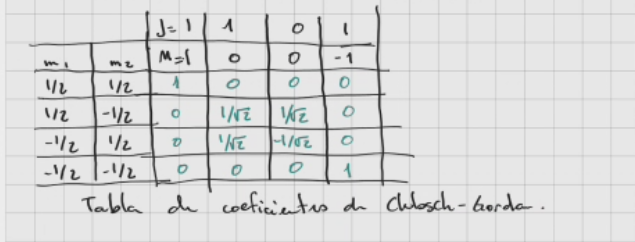
\includegraphics{Graficas/G1-Aug9.png}


\subsection{Consecuencias en el espectro de $\hat{H}$}

Los niveles de energía de la partícula compuesta están dados por el espectro de $\hat{H}$ que tiene entonces $2$ niveles de energía: $E_j=0$, $E_j=1$ de multiplicidad $1$ y $3$ respectivamente.

Por ejemplo, para $\hat{H}=K \vec{S}_1\cdot\vec{S}_2=k\frac{1}{2}\vec{S}^2-\vec{S}_1^2-\vec{S}_2^2$

Autovectores: singlete y los vectores del triplete.

\begin{align*}
    \hat{H}\left(\frac{1}{\sqrt{2}}\left(\ket{+-}-\ket{-+}\right)\right)&=\\
    &\vdots\\
    &=\frac{K}{\sqrt{2}}\left(\frac{3}{4}\hbar^2\ket{-+}-\frac{3}{4}\hbar^2\ket{+-}\right)
\end{align*}

$E_{J=0}=-\frac{3}{4}K\hbar^2$

$E_{J=1}=\frac{1}{4}K\hbar^2$

Démonos cuenta que diagonalizamos al operador 


\subsubsection{Aplicación}
La línea de $21cm$ del hidrógeno. 

En el caso del átomo de hidrógeno, el estado $1s$ está formado por 4 estados dados por la interacción entre los espines del electrón y el protón.

La diferencia de energía aquí: $\Delta E = E_1-E_o=6E-6eV$

a esto le llamamos la estructura hiperfina del estado $1s$.

Si un átomo de hidrógeno se encuentra en el estado de energía $E_1$, este no es por fuerza un estado estacionario por interacción con el campo electromagnético y se desexcita al estado fundamental $E_o$ por emisión espontánea con vida media muy larga: $\tau \approx 10E7\hat{a}$

El fotón producido es de energía $\Delta E $ al cual le corresponde una longitud de onda $\lambda=21cm$.

En el gas interestelar formado por hidrógeno, las colisiones entre átomos son responsables de una temperatura $\tau\approx100K\Rightarrow k_bT=10E-2eV$

\subsection{Descomposición general de momenta angulares:}

Ver cómo se acoplan 2 partículas con momentum angular $j_1$ y $j_2$. Están interactuando por medio de un hamiltoniano $\hat{H}$ que es invariante ante rotaciones globales del sistema.


Niveles de energía corresponden a las reprecentaciones irreducibles del grupo de rotación $D_j$. 

\textbf{Objetivo:} saber cómo el espacio de Hilbert se descompone en representaciones irreducibles $D_J$:


\begin{align*}
    D_{j_1}\otimes D_{j_2}=\bigoplus_{J=\abs{j_1-j_2}}D_J
\end{align*}



\subsubsection{Aplicación: simetría de isoespín}
Veamos la utilidad de los coeficientes de Clebsch-Gordon para:

$$
    D_1\otimes D_{1/2}=D_{J=\frac{1}{2}}\oplus D_{J=3/2}
$$

No vamos a aplicar simetría rotacional, sino la de sioesín, de física nuclear, es la del grupo $SU(2)$.

Poniendo en un lado el valor de la carga eléctrica $Q$, el protón y el neutrón tienen propiedades muy similares:

$m_n=940MeV$

$m_p=939Mev$

y se comportan de manera muy similar con las interacciones nucleares.

\textbf{1930}: Heisenberg hace una hipótiesis: el protón y el neutrón tienen la misma naturaleza: son la misma partícula: nucleón.

La carga positiva, o la carga neutra corresponden a 2 estados disntintos: $\ket{p},\ket{n}$ esto sería un grado de libertad más.

El estado de un nucleón está descrito por un espacio de dimensión 2 cuya base: $\ket{p},\ket{n}$:$D_{j=1/2}$.

Dado que la fuerza nuclear no distingue entre protones y neutrones, Heisenberg postula que la fuerza nuclear tiene una simetría respecto a la mezcla de estos dos estados.
$\Rightarrow$ hay una invarianza por el grupo $SU(2)$.

A esta invarianza se le conoce como simetría de isoespín.

Unicamente, la fuerza electromagnética hace la distinción entre los dos estados. Esta fuerza rompe la simetría. Pero, la fuerza electromangética es mucho menor a la fuerza nuclear, eso explicaría en la visión de Heisenberg, la diferencia de masas.

En el espaicio $D_{1/2}$ el operador de carga eléctrica sería:

\begin{align*}
    \hat{Q}=\begin{pmatrix}
        1&0\\0&0
    \end{pmatrix}
\end{align*}

Otras partículas nucleares han sido descubiertas, los piones, $\pi^+,\pi^0,\pi^-$ de cargas respectivas $+1,0,-1$.

En la hipótesis de Heisenberg, estas serían la misma partícula: el pión.

Tendríamos 3 posibilidades $\Rightarrow D_{j=1}$ de dimensión 3.

Es la fuerza electromagnética la responsable de distinguir entre $\ket{\pi^{\pm,0}}$.

\textbf{Reacciones entre piones y nucleones:}

$p+\pi^-\rightarrow n +\pi^0$

Resulta que considerar a la simetría de isoespín, permite el cálculo de secciones eficaces.

La sección eficaz es proporcional a la probabilidad de la reacción:

\begin{align*}
    \sigma(N+\pi\rightarrow N'+\pi')=\abs{\bra*{N',\pi'}\hat{U}\ket*{N,\pi}}^2
\end{align*}

$\hat{U}$ es un operador de difusión.

\textit{Ejercicio:}

1. Un estado $\ket{N,\pi}$ se describe por un vector en el espacio 



\subsubsection{Reglas de selección y el teorema de Wigner-Eckardt}
Aplicación del momentum angular en espectroespín.

Considerar a un átomo aislado sometido a una onda electromagnética plana de frecuencia $\omega$.

Por teoría de perturbaciones, vemos que hay transiciones entre los orbitales $(n,l,m)$, absorbiendo o emitiendo un fotón.

La probabilidad de transición de $a=(n,l,m)$ hacia $b=(n',l',m')$ está dada por:

\begin{align*}
    P_{a\rightarrow b}(t)\approx \frac{I}{2\epsilon_oc\hbar^2}\abs{D_{ba}}^2\cos^2\theta F(t,\omega_{ba}\pm \omega)
\end{align*}

\begin{align*}
    \abs*{D_{ba}}^2= l^2\abs{\bra*{n',l',m'}\vec{x}\ket{n,l,m}}^2
\end{align*}

\textbf{Regla de selección:}

Aunque los estados cuánticos orbitales $(n,l,m)$ son, por lo general, difíciles de calcular en un átomo con varios electrones,
un simple argumento de simetría, llamado regla de selección muestra que el elemento de matriz es nulo excepto cuando $l'=l\pm 1$

Las transiciones posibles en el espectro atómico:

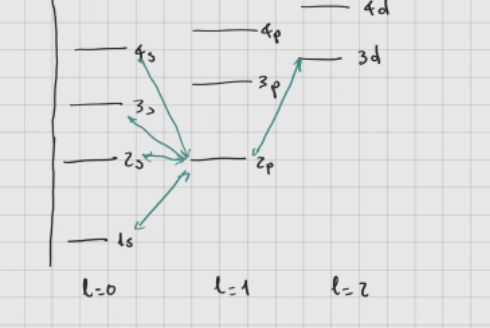
\includegraphics[width=0.4\textwidth]{Graficas/Aug19-1.png}

El elemento de matriz hace que intervengan 3 objetos que pertenecen a representaciones irreducibles de $SO(3)$:

\begin{align*}
    \ket{n,l,m}&\in D_l\\
    \ket{n',l',m'}&\in D_l'\\
\end{align*}

Y el operador $\vec{x}\in D_1$

El elemento de matriz es el producto interno entre los vectores $$\vec{x}\ket{n,l,m}\in D_1\otimes D_l=D_{l-1}\otimes D_{l}\otimes D_{l+1}$$

Y del vector
$$ \ket{n',l',m'}\in D_{l'}$$

Dado que vectores que pertenecen a rep irreducibles distintas son ortogonales, para que el elemento de matriz no sea cero:
\begin{align*}
    l'&=l-1&l'&=l&l'&=l+1
\end{align*}

El caso $l=l'$ se excluye por otra simetría, la simetría de paridad, gupo $\mathbb{Z}_2={\mathbb{1,-1}}$

Es una simetría en el átomo ya que $V(\vec{x})=V(-\vec{x})$.

El operador $\vec{x}$ es impar (paridad -1) y $\ket{n,l,m}$ es de paridad $(-1)^2$.

\subsubsection{Teorema de Wigner-Eckardt}

\textbf{Definiciones:}

\begin{itemize}
    \item \textbf{Operador vectorial} es un conjunto de operadores $\vec{O}=(O_1,O_2,O_3)$ sobre el cual una rotación lo transforma en un vector en $D_{l=1}$
    \item \textbf{Operador escalar} es un operador invariante bajo el efecto de rotaciones.
    \item \textbf{Operador tensorial irreducible} de rango $j$ es un conjunto de $2j+1$ operadores denotados por $T_j:=(T_{j,m''})_{m''=-j\rightarrow j}$ sobre el cual actúa el grupo $SO(3)$ de rotaciones (o $SU(2)$) y que se transforma como un vector de $2j+1$ componentes de la rep irreducible $D_j$.
    \item \textbf{Operador tensorial} es un cojunto de operadores sobre el cual actúa $SO(3)$ o $SU(2)$ y que bajo el efecto de una rotación, se transforma como un vectore de una reprresentación del gurpo de rotación (no por fuerza irreducible).
\end{itemize}

\textbf{Teorema} Si $D_l'$ no está presente en la descomposición 

$$
D_l''\otimes D_l = \bigoplus_{\abs*{l-l''}}^{\abs{l+l''}}D_k
$$
 entonces los elementos de matriz son nulos (regla de selección)

 Si $D_{l'}$ está presente en la descomposición entonces el elemento de matriz en cuestión es no nulo y se expresa gracias a los coeficientes de Clebsch-Gordon.

 

 \chapter{Métodos de aproximación}

 \textbf{Interés:}
 \begin{itemize}
     \item Muchas veces son indispensables, sin estos, el problema puede ser irresoluble.
     \item Algunas veces permiten entender mejor fenómenos simples.
 \end{itemize}

 \textbf{Dos tipos de problemas:}

 \begin{enumerate}
     \item Problemas estacionarios: $\hat{H}$ independiente del tiempo. Objetivo: calcular el espectro de $\hat{H}$. (idea: resolver el estado fundamental: método variacional.)
     \item Problema de evolución: Tenemos $\psi(0)\rightarrow$ calcular la evolución a $\psi(t)$.
 \end{enumerate}


\section{Teoría de perturbaciones estacionarias:}

\textbf{Idea:} 

$$\hat{H}=\hat{H}_o+\lambda\hat{H}_1$$

$\lambda$ pequeño, $H_1$ se le conoce como perturbación

Resolvemos por medio de series de potencias en $\lambda$.

\textbf{Objetivo:} Encontrar el espectro de $\hat{H}$

\begin{align*}
    \hat{H}\ket{\psi_n(\lambda)}=E_n(\lambda)\ket{\psi_n(n)}
\end{align*}

Notemos que $\hat{H}(0)=\hat{H}_o$ es un hamiltoniano del cual conocemos el espectro.



$\hat{H}_1$ es un operador llamado perturbación del cual conocemos los elementos de matriz en la base $\{\ket{n}\}$:

\begin{align*}
    \bra{n'}H_1\ket{n}, ~~~ n,n'\geq 0
\end{align*}

Buscamos entonces calcular los autovalores $E_n(\lambda)$ y las componentes de los autovectores $\ket{\psi_n(\lambda)}$ en la base $\{\ket{n}\} $ para $\lambda<<1$.

\textbf{Nota:} puede ser que se de la igualdad en:

\begin{align*}
    \epsilon_o\leq\epsilon_1\leq\cdots
\end{align*}
En particular aquí $\epsilon$ es un degenerado de multiplicidad $N$.

\subsection{Caso no degenerado:}
\textbf{Proposición:} Si $\epsilon_n$ es un autovalor no-degenerado de $H_o$ (n fijo) entonces para $\lambda<<1$.

\begin{align*}
    E_n(\lambda)&=\epsilon_n+\lambda E^{(1)}+\lambda^2E^{(2)}+\cdots\\
    \ket{\psi_n(\lambda)}&= \ket{n}+\lambda\ket{\psi^{(1)}}+\lambda^2\ket{\psi^{(2)}}+\cdots
\end{align*}

donde la corrección de primer orden:

\begin{align*}
    E^{(1)}&=\bra{n}H_1\ket{n}:\text{ corrección de primer orden de la energía.}\\
    \bra{n'}\ket*{\psi^{(1)}}&=\frac{\bra{n}H_1\ket{n}}{\epsilon_n-\epsilon_{n'}}\text{: corrección a primer orden del estado.}
\end{align*}

Y a segundo orden:

\begin{align*}
    E^2=\sum_{n'\neq n}\frac{\abs*{\bra{n'}H_1\ket{n}}^2}{\epsilon_n-\epsilon_{n'}}
\end{align*}

\textbf{Nota:} El vector $\ket{\psi^(1)}$ está expresado por componentes:
\begin{align*}
    \ket{\psi^{(1)}}=\sum_{n'\neq n}\ket{n'}\bra{n'}\ket{\psi^{(1)}}=\sum_{n'\neq n}\ket{n'}\bra{n'}H_1\ket{n}/(\epsilon_n-\epsilon_{n'})
\end{align*}

Para el nivel de energía fundamental, $\epsilon_o$, tenemos que $(\epsilon_o-\epsilon_{n'})<0\Rightarrow E^{(2)}\leq 0$

\textbf{Prueba:} Expandir la ecuación de Schrodinger en series de potencias. Y agrupar por los órdenes de lambda. Aplicar un ket $n$ o $n'$ y ``despejar''.

\textbf{Ejemplo:} vibración anharmónica de un átomo:

\begin{align*}
    \hat{H}=\frac{\vec{p}^2}{2m}+\frac{1}{2}kx^2+\lambda x^4
\end{align*}

Aquí $H_o$ es el oscilador armónico y $\lambda H_1$ la perturbación.

\begin{figure}[H]
    \centering
    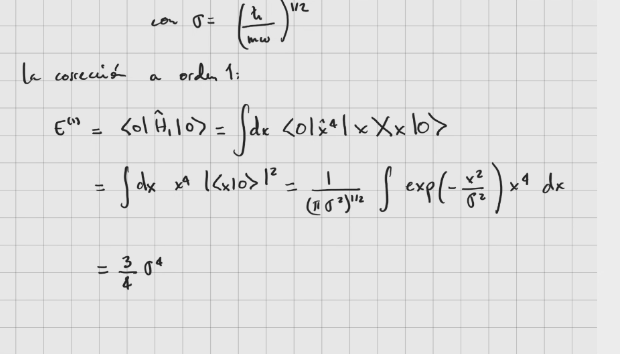
\includegraphics[width=0.5\textwidth]{Graficas/Aug23-1.png}
\end{figure}

\begin{figure}[H]
    \centering
    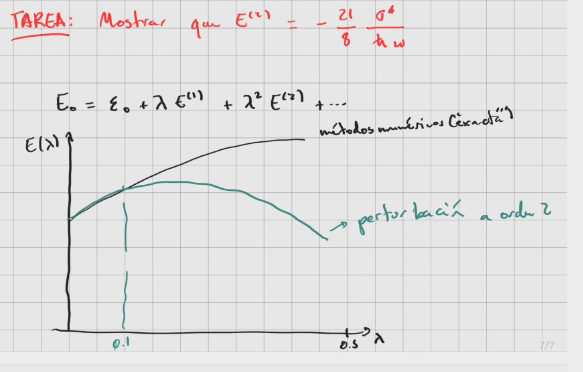
\includegraphics[width=0.5\textwidth]{Graficas/Aug23-2.png}
\end{figure}

\subsubsection{Interacción espín-orbita}

\begin{align}
    H'_{SO}=\left(\frac{e^2}{8\pi\epsilon_0}\right)\frac{1}{m^2c^2r^3}\vec{S}\cdot\vec{L}
\end{align}

este hamiltoniano no conmuta con $\vec{S}$ y $\vec{L}$ por separado, pero si con $\vec{S}^2$ y $\vec{L}^2$ y con $\vec{J}=\vec{L}+\vec{S}$

Quiere decir que $\vec{J}$,$\vec{S}^2$,$\vec{L}^2$ se conservan.

Analicemos a $\vec{J}^2$:

\begin{align*}
    \vec{L}\cdot\vec{S}=\frac{1}{2}\left(\vec{J}^2-\vec{L}^2-\vec{S}^2\right)
\end{align*}

Los autovalores son $\vec{L}\cdot\vec{S}$ son

\begin{align*}
    \frac{\hbar^2}{2}\left[j(j+1)-l(l+1)-s(s+1)\right]
\end{align*}

Con $s=1/2$ y el valor esperado de $1/r^3$ es 

\begin{align*}
    < \frac{1}{r^3} > = \frac{1}{l(l+1/2)(l+1)n^3a^3}
\end{align*}


entonces

\begin{align*}
    E^1_{SO}=
\end{align*}

\section{Principio variacional:}

Método de aproximación: sirve para estimar el estado fundamental.

\subsection{Repaso: Multiplicadores de Lagrange}

Sea $f({x_k})$ una función con $K$ variables relacionadas por un conjunto de $J$ restricciones $g_j({x_k})=a_j$.
Buscar los puntos ${x_k}$, extremos de $f$ que satisfagan las restricciones.

\begin{align*}
    \dd{f}=\sum_{i=0}^K\pdv*{f}{x_i}\dd x_i = 0 && \dd g_i=\sum_{i=0}^K\dv*{g_i}{x_i}\dd x_i=0
\end{align*}

con $j=1,2,\cdots$

\subsubsection{Procedimiento general}

Formar la combinación 


\subsection{Teoría}

\subsubsection{Teorema:} $E_0\leq $

\chapter{Estadística cuántica}

\subsection{Descripción de un ensamble estadístico de estados cuánticos por el operador densidad}

\subsection{Definición del operador Densidad}

En mecánica clásica, en principio, podemos conocer totalmente a un sistema. Ya que está regido por leyes deterministas (podemos conocer su pasado y su futuro).

Pero, hay sistemas caóticos (sensibles a condiciones iniciales). $\Rightarrow$ este determinismo sea un poco iluso. Se considera al caos como una fuente de azar.

$\Rightarrow$ se requiere de una descripción probabilística de un sistema, aún con pocos grados de libertad.

En el caso más sencillo, donde tenemos a los estados de una partícula $(\vec{x}_i,\vec{p}_i)$ cada uno con probabilidad $P_i$ y $\sum_i P_i =1$, o bien usando una distribución de probabilidad, $P(\vec{x},\vec{p})$ en el espacio de fases para describir de forma probabilística del estado de una partícula.

Esto es un ensamble de estados clásicos.

\bigskip

\textbf{Contraparte cuántica:}

Un sistema cuántico tiene otra componente de azar $\rightarrow$ interacción con el ambiente. Este azar es intrínseco de la naturaleza.

\bigskip

\textbf{El postulado de la medición}

Una partícula cuántica se describe por un $\psi\in\mathbb{H}$. Si $\hat{A}$ es un operador (autoadjunto) asociado a un observable, cuyo espectro es $(a_j)_j$. Entonces la medición de $A$ en el estado $\psi$ tiene como resultado $a_j$ con probabilidad:

\begin{align*}
    P_\psi(a_j)=\frac{\abs{\abs{P_j\psi}}^2}{\abs{\abs{\psi}}^2}=\frac{\bra{\psi}P_j\ket{\psi}}{\bra{\psi}\ket{\psi}}
\end{align*}

$P_j$ es el proyector espectral sobre el espacio propio $a_j$. Podemos vlover a formular el postulado de la medición:

\bigskip

\textbf{Postulado de la medición}

Luego de una medición, el sistema cuántico $\psi$ está descrito por la superposición estadística de estados $P_j\psi$ cada una con probabilidad:

\begin{align*}
    P_\psi(a_j)=\frac{\abs{\abs{P_j\psi}}^2}{\abs{\abs{\psi}}^2}=\frac{\bra{\psi}P_j\ket{\psi}}{\bra{\psi}\ket{\psi}}
\end{align*}

Insistir en el hecho que estas probabilidades $P_\psi(a_j)$ para todos los observables $\hat{A}$ caracterizan al sistema físico, en el sentido que son los valores accesibles experimentalmente y es la única forma de contrastar el experimento con la teoría.

Valor esperado:

\begin{align*}
    A _\psi = \sum_j P_\psi (a_j)\cdot a_j=\frac{\bra{\psi}A\ket{\psi}}{\bra{\psi}\ket{\psi}}
\end{align*}

Queremos estudiar la posibilidad de que exista también una componente de azar del desconocimiento del sistema.

En vez de considerar a un único estado cuántico $\psi\in\mathcal{H}$ queremos considerar a un ensamble estadístico de estados. $\psi_j\in\mathcal{H}$ con probabilidad $p_i$ tales que la suma es $1$.

Por el postulado de la medición, para medir $a\hat{A}$ en el valor $a_j$

\begin{align*}
    p(a_j)=\sum_i p_ip_\psi(a_j)
\end{align*}

\begin{align*}
    A = \sum_i p(a_j)a_j=\sum_i p_i \frac{\bra{\psi_i}A\ket{\psi_i}}{\bra{\psi_i}\ket{\psi_i}}
\end{align*}

Esta presencia de 2 fuentes de azar es incómoda, esta definición permite simplificar el formalismo.

\bigskip

\textbf{Definición:} Para un ensamble estadístico de los estados $\psi_i\in\mathcal{H}, i=1,2,3,\cdots$ con probabilidades respectivas $p_i$, al operador densidad asociado es:

\begin{align*}
    \hat{\rho}&:=\sum_i P_iP_{\psi_i}&
\end{align*}


También conocido como matriz densidad o estado cuántico, donde $P_j$ es el proyector ortogonal de rango 1 sobre el estado $\psi_i$.

En el caso particular de un solo estado, $\psi$